\section{Hạn chế và Cầu nối sang Học sâu}
\label{sec:limitations_and_bridge_to_deep_learning}

Kỷ nguyên của các đặc trưng thủ công là một chương vàng son trong lịch sử thị giác máy tính. Các thuật toán như SIFT, HOG, và các phương pháp biểu diễn như Fisher Vector là những thành tựu kỹ thuật đáng kinh ngạc, minh chứng cho sự sáng tạo và hiểu biết sâu sắc của con người về bản chất của tín hiệu hình ảnh. Chúng đã đặt nền móng cho vô số ứng dụng và định hình nên tư duy của cả một thế hệ nhà nghiên cứu.

Tuy nhiên, cũng chính trong quá trình đẩy các phương pháp này đến giới hạn của chúng, cộng đồng khoa học đã nhận ra những bức tường vô hình, những hạn chế cố hữu không thể vượt qua chỉ bằng cách thiết kế các bộ lọc thông minh hơn. Những hạn chế này không phải là lỗi của các thuật toán, mà là giới hạn của chính triết lý "thiết kế thủ công". Phần này sẽ phân tích các bức tường đó và chỉ ra con đường tất yếu dẫn đến cuộc cách mạng học sâu.

\subsection{Khó khăn trong Biến đổi Scale, Ánh sáng và Góc nhìn}
\label{subsec:transformation_challenges}

Mặc dù các đặc trưng thủ công được thiết kế với mục tiêu đạt được tính bất biến, khả năng của chúng bị giới hạn bởi các mô hình toán học đơn giản hóa về thế giới thực.

\subsubsection{Biến đổi Góc nhìn 3D và Phép chiếu Phối cảnh}
\label{subsubsec:viewpoint_limitations}
Đây có lẽ là hạn chế nghiêm trọng nhất. Các bộ mô tả như SIFT và SURF được xây dựng dựa trên giả định rằng các biến đổi cục bộ trên một vùng ảnh có thể được xấp xỉ bằng một \textbf{phép biến đổi affine}. Phép biến đổi này bao gồm tịnh tiến, xoay, co giãn, và cắt xiên (shear). Nó là một xấp xỉ tốt khi một bề mặt phẳng được nhìn từ các góc độ hơi khác nhau.

Tuy nhiên, thế giới thực là 3D, và quá trình máy ảnh ghi lại hình ảnh tuân theo quy luật của \textbf{phép chiếu phối cảnh (perspective projection)}. Dưới phép chiếu này, các đường thẳng song song trong thế giới 3D sẽ hội tụ tại một điểm trong ảnh, và các hình vuông có thể trở thành hình thang. Phép biến đổi này là phi tuyến và không thể được mô tả chính xác bằng một phép biến đổi affine, đặc biệt là khi có sự thay đổi góc nhìn lớn hoặc khi đối tượng không phẳng.

\begin{center}
	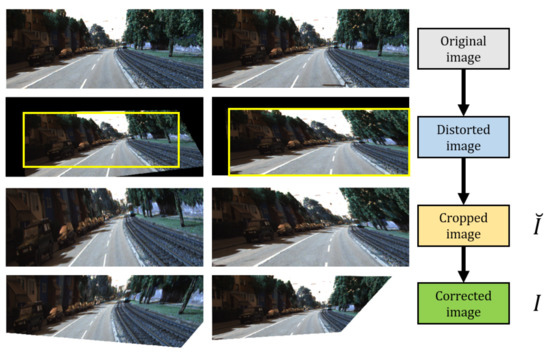
\includegraphics[width=0.8\textwidth]{images/sift_perspective_distortion_failure.jpg}
	\captionof{figure}{Sự thất bại của giả định affine dưới phép chiếu phối cảnh mạnh. Vùng ảnh xung quanh một điểm đặc trưng trên bề mặt phẳng nhìn trực diện (trái) sẽ bị biến dạng thành một hình thang khi nhìn từ một góc xiên (phải). Các biểu đồ hướng gradient bên trong sẽ thay đổi hoàn toàn, làm cho bộ mô tả SIFT không thể so khớp được.}
	\label{fig:sift_perspective_failure}
\end{center}
% Keyword gợi ý: sift perspective distortion, affine vs projective transformation, feature matching failure viewpoint

Khi một vùng ảnh bị biến dạng phối cảnh mạnh, cấu trúc gradient bên trong nó bị thay đổi một cách phi tuyến, khiến cho các biểu đồ hướng (cả trong SIFT và HOG) không còn ổn định. Kết quả là, hai vùng ảnh mô tả cùng một bề mặt 3D nhưng được chụp từ hai góc nhìn rất khác nhau sẽ tạo ra hai vector đặc trưng hoàn toàn khác biệt, dẫn đến việc so khớp thất bại.

\subsubsection{Biến đổi Ánh sáng Phức tạp}
\label{subsubsec:illumination_limitations}
Các đặc trưng thủ công cố gắng đạt được tính bất biến với ánh sáng thông qua các kỹ thuật chuẩn hóa. Ví dụ, SIFT chuẩn hóa L2 vector mô tả 128-D của nó; HOG chuẩn hóa các vector trong từng khối (block).

Các phương pháp này hoạt động tốt dưới các giả định về \textbf{thay đổi ánh sáng tuyến tính và toàn cục}, tức là khi toàn bộ vùng ảnh trở nên sáng hơn hoặc tối hơn, hoặc có độ tương phản cao hơn hoặc thấp hơn một cách đồng đều. Tuy nhiên, các điều kiện ánh sáng trong thực tế phức tạp hơn nhiều:
\begin{itemize}
	\item \textbf{Bóng đổ (Cast Shadows):} Một cái bóng sắc nét đổ qua một vật thể có thể tạo ra các cạnh giả cực mạnh, lấn át các cạnh thực của vật thể.
	\item \textbf{Phản xạ và Lóe sáng (Specular Highlights):} Một điểm lóe sáng trên bề mặt kim loại hoặc nhựa bóng có thể làm "cháy" một vùng pixel, xóa sạch mọi thông tin về kết cấu bên dưới.
	\item \textbf{Thay đổi màu sắc nguồn sáng:} Cùng một vật thể sẽ trông rất khác dưới ánh sáng mặt trời, ánh đèn huỳnh quang, hay ánh nến. Các đặc trưng dựa trên cường độ ảnh xám như SIFT và HOG rất nhạy cảm với những thay đổi này.
	\item \textbf{Chiếu sáng cục bộ và phi đồng nhất:} Ánh sáng trong một cảnh hiếm khi đồng đều. Các hiệu ứng như vinette (vùng tối ở góc ảnh) hay ánh sáng chiếu từ một phía có thể làm thay đổi đáng kể độ lớn của gradient trên toàn bộ vật thể.
\end{itemize}

\begin{center}
	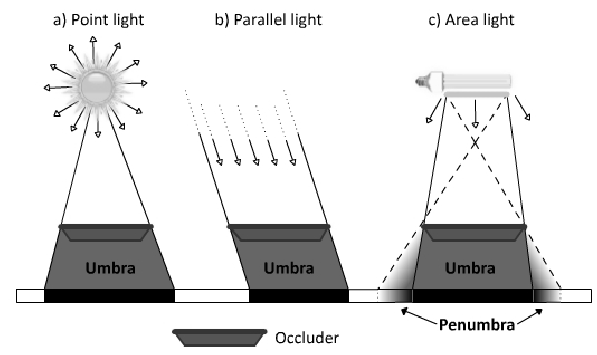
\includegraphics[width=0.7\textwidth]{images/hard_shadow_illumination_problem.png}
	\captionof{figure}{Ví dụ về điều kiện ánh sáng phức tạp. Bóng đổ sắc nét tạo ra các cạnh giả, trong khi các vùng phản xạ chói lóa làm mất thông tin kết cấu. Các phương pháp chuẩn hóa đơn giản không thể xử lý hiệu quả các hiện tượng phi tuyến và cục bộ này.}
	\label{fig:hard_shadow_problem}
\end{center}
% Keyword gợi ý: hard shadow computer vision, illumination challenges vision, specular highlight problem

\subsection{Giới hạn Hiệu năng và Tính Tổng quát}
\label{subsec:performance_generalization_limits}

Ngoài việc mong manh trước các biến đổi vật lý, triết lý thiết kế thủ công còn vấp phải hai giới hạn cơ bản hơn: một ngưỡng hiệu năng không thể vượt qua và khả năng khái quát hóa kém.

\subsubsection{Sự bão hòa về Hiệu năng và ''Vực thẳm Ngữ nghĩa''}
\label{subsubsec:performance_plateau}
Vào cuối những năm 2000 và đầu những năm 2010, hiệu năng của các hệ thống thị giác máy tính trên các bộ dữ liệu tiêu chuẩn đã có dấu hiệu chững lại. Ví dụ, trong cuộc thi Nhận dạng Hình ảnh Quy mô lớn ImageNet (ILSVRC), tỷ lệ lỗi của các hệ thống tốt nhất, thường dựa trên Fisher Vector và SVM, đã bị kẹt ở mức khoảng 25-28\%. Mọi nỗ lực tinh chỉnh các bộ trích xuất đặc trưng hay các phương pháp mã hóa chỉ mang lại những cải thiện rất nhỏ.

\begin{center}
	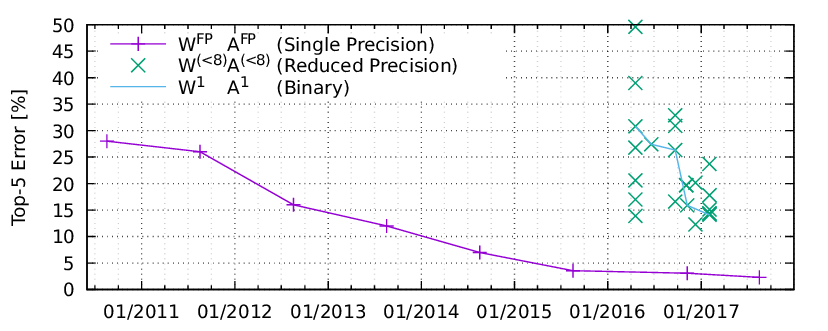
\includegraphics[width=0.9\textwidth]{images/imagenet_error_rate_over_time.png}
	\captionof{figure}{Tỷ lệ lỗi top-5 trên cuộc thi ImageNet (ILSVRC) qua các năm. Có thể thấy một sự chững lại về hiệu năng của các phương pháp cổ điển trước năm 2012, và sau đó là một bước nhảy vọt đột ngột với sự xuất hiện của AlexNet (một mạng CNN sâu).}
	\label{fig:imagenet_error_rate}
\end{center}
% Keyword gợi ý: imagenet error rate over time, alexnet performance jump, ilsvrc results history

Nguyên nhân sâu xa của sự bão hòa này là \textbf{"vực thẳm ngữ nghĩa" (semantic gap)}: khoảng cách khổng lồ giữa thông tin mức thấp mà các đặc trưng thủ công nắm bắt được (cạnh, góc, kết cấu, màu sắc) và các khái niệm ngữ nghĩa mức cao mà con người sử dụng để diễn giải một hình ảnh (vật thể, hành động, khung cảnh).
Các đặc trưng như SIFT hay HOG không "hiểu" một "bánh xe" là gì; chúng chỉ thấy một tập hợp các đường cong và đường thẳng. Do đó, chúng rất dễ bị đánh lừa. Một bức tường gạch có thể có nhiều "góc" Harris hơn một khuôn mặt người. Một con chó đốm trên nền tuyết lốm đốm là một cơn ác mộng cho các bộ mô tả dựa trên kết cấu.

\subsubsection{Khả năng Tổng quát hóa Kém và Chi phí Thiết kế}
\label{subsubsec:poor_generalization}
Do được thiết kế dựa trên các giả định về các loại cấu trúc hình ảnh, các đặc trưng thủ công thường rất chuyên biệt cho một loại tác vụ hoặc một lĩnh vực dữ liệu nhất định.
\begin{itemize}
	\item Một bộ mô tả HOG được tối ưu hóa để phát hiện người đi bộ (vốn có hình dạng thẳng đứng đặc trưng) sẽ hoạt động rất kém để phát hiện ô tô hoặc máy bay.
	\item Các đặc trưng SIFT/SURF hoạt động tốt trên các vật thể có kết cấu phong phú, nhưng lại thất bại trên các bề mặt trơn nhẵn, không có kết cấu.
	\item Việc áp dụng các phương pháp này sang một lĩnh vực mới, ví dụ như phân tích ảnh y khoa hoặc ảnh viễn thám, đòi hỏi một quá trình nghiên cứu và thiết kế lại đặc trưng vô cùng tốn kém, thường là công sức của cả một luận án tiến sĩ.
\end{itemize}
Hiệu suất của toàn bộ hệ thống bị giới hạn bởi sự thông minh của người thiết kế ra bộ trích xuất đặc trưng. Con người chỉ có thể mã hóa những gì chúng ta có thể mô tả một cách hình thức. Đây chính là "nút thắt cổ chai" lớn nhất của kỷ nguyên cổ điển.

\subsection{Vai trò Lịch sử: Chuẩn bị cho sự bùng nổ CNN}
\label{subsec:historical_role_cnn_bridge}

Nhìn lại, kỷ nguyên của các đặc trưng thủ công không phải là một thất bại, mà là một bước đệm không thể thiếu, một người thầy vĩ đại đã dạy cho chúng ta những bài học vô giá và đặt ra những câu hỏi đúng đắn, chuẩn bị cho cuộc cách mạng sắp tới. Các mạng nơ-ron tích chập (CNN) không xuất hiện từ hư không; chúng chính là câu trả lời cho những vấn đề mà các phương pháp cổ điển đã chỉ ra, và về bản chất, chúng là sự tự động hóa và tổng quát hóa các nguyên lý đã được khám phá trong kỷ nguyên thủ công.

Đây là những di sản quan trọng nhất:
\begin{description}
	\item[Tư duy về Đặc trưng Phân cấp (Hierarchical Features):] Các phương pháp cổ điển đã cho thấy sức mạnh của việc xây dựng các biểu diễn từ đơn giản đến phức tạp: từ pixel $\rightarrow$ gradient $\rightarrow$ biểu đồ hướng (SIFT/HOG) $\rightarrow$ histogram từ thị giác (BoVW). CNN đã đưa ý tưởng này lên một tầm cao mới. Các lớp đầu tiên của một mạng CNN tự động học được các bộ lọc phát hiện cạnh và màu sắc, rất giống với các bộ lọc Gabor hay các phép toán gradient thủ công. Các lớp sâu hơn kết hợp các đặc trưng đơn giản này lại để tạo ra các đặc trưng phức tạp hơn, tương ứng với các bộ phận của vật thể, và cuối cùng là toàn bộ vật thể.
	
	\begin{center}
		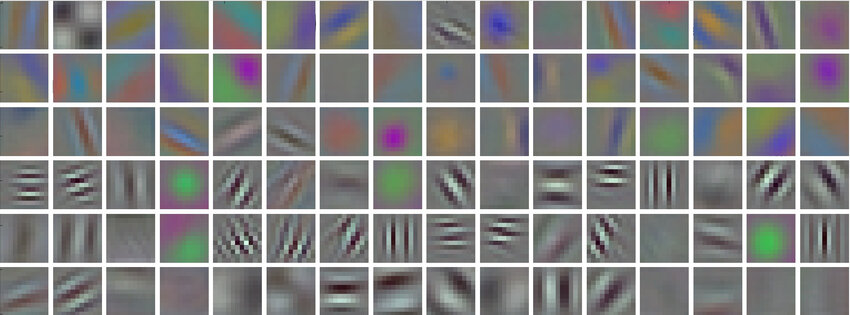
\includegraphics[width=0.9\textwidth]{images/cnn_first_layer_filters.png}
		\captionof{figure}{Trực quan hóa các bộ lọc được học bởi lớp tích chập đầu tiên của mạng AlexNet. Có thể thấy rõ các bộ lọc phát hiện cạnh ở nhiều hướng khác nhau và các bộ lọc phát hiện đốm màu, tương tự như các khối xây dựng cơ bản trong xử lý ảnh cổ điển.}
		\label{fig:cnn_first_layer_filters}
	\end{center}
	% Keyword gợi ý: cnn first layer visualization, alexnet filters, gabor filter cnn
	
	\item[Tầm quan trọng của Tính Bất biến:] Nỗi ám ảnh của kỷ nguyên thủ công về tính bất biến với tỷ lệ, xoay, và tịnh tiến đã được kế thừa bởi kiến trúc CNN. Các phép toán như \textbf{tích chập (convolution)} cung cấp tính bất biến với tịnh tiến, trong khi \textbf{gộp (pooling)} cung cấp một mức độ bất biến cục bộ với các biến dạng nhỏ. Thay vì được lập trình cứng, các tính bất biến này được học một cách mềm dẻo từ dữ liệu thông qua quá trình huấn luyện.
	
	\item[Tối ưu hóa End-to-End:] Pipeline cổ điển bao gồm nhiều bước rời rạc (phát hiện đặc trưng, mô tả đặc trưng, mã hóa, phân loại) được thiết kế và tối ưu hóa một cách độc lập. CNN đã hợp nhất tất cả các bước này vào một kiến trúc duy nhất, có thể tối ưu hóa \textbf{một cách toàn diện (end-to-end)} bằng thuật toán lan truyền ngược (backpropagation). Mọi thành phần của mạng, từ các bộ lọc ở lớp đầu tiên đến bộ phân loại ở lớp cuối cùng, đều được điều chỉnh đồng thời để tối thiểu hóa một hàm mất mát duy nhất cho tác vụ cuối cùng. Đây chính là lợi thế lớn nhất và là nguồn sức mạnh phi thường của học sâu.
\end{description}

Tóm lại, những thách thức không thể vượt qua của đặc trưng thủ công đã tạo ra một nhu cầu cấp thiết cho một phương pháp mới có thể \textbf{tự học các biểu diễn} trực tiếp từ dữ liệu, thay vì phải thiết kế chúng bằng tay. Nó cần phải có khả năng học các đặc trưng phân cấp, có tính bất biến, và có thể được tối ưu hóa một cách toàn diện. Câu trả lời cho tất cả những yêu cầu này chính là Mạng Nơ-ron Tích chập.

Khi lật sang chương tiếp theo, chúng ta không phải đang từ bỏ quá khứ, mà là đang đứng trên vai của những người khổng lồ để nhìn xa hơn. Chào mừng bạn đến với kỷ nguyên của học sâu.

\section*{Tài liệu tham khảo}
\begin{itemize}
	\item[1] Russakovsky, O., Deng, J., Su, H., Krause, J., Satheesh, S., Ma, S., ... \& Fei-Fei, L. (2015). ImageNet Large Scale Visual Recognition Challenge. \textit{International Journal of Computer Vision}, \textit{115}(3), 211-252. (Cung cấp bối cảnh về cuộc thi ILSVRC và kết quả của các phương pháp trước và sau kỷ nguyên học sâu, minh họa cho sự chững lại về hiệu năng).
	\item[2] Krizhevsky, A., Sutskever, I., \& Hinton, G. E. (2012). ImageNet classification with deep convolutional neural networks. In \textit{Advances in neural information processing systems (NIPS)}. (Paper bản lề giới thiệu AlexNet, thể hiện bước nhảy vọt về hiệu năng so với các phương pháp dựa trên đặc trưng thủ công và chính thức khởi đầu kỷ nguyên học sâu trong thị giác).
	\item[3] Zeiler, M. D., \& Fergus, R. (2014). Visualizing and understanding convolutional networks. In \textit{European conference on computer vision (ECCV)}. (Bài báo kinh điển về việc trực quan hóa các bộ lọc trong CNN, cho thấy mối liên hệ giữa các đặc trưng học được ở lớp đầu và các bộ lọc cạnh/màu sắc cổ điển).
	\item[4] Perronnin, F., Sánchez, J., \& Mensink, T. (2010). Improving the Fisher Kernel for large-scale image classification. In \textit{European Conference on Computer Vision (ECCV)}. (Một ví dụ tiêu biểu cho các phương pháp state-of-the-art dựa trên đặc trưng thủ công ngay trước khi AlexNet xuất hiện, đại diện cho "đỉnh cao" của kỷ nguyên cũ).
	\item[5] Hartley, R., \& Zisserman, A. (2003). \textit{Multiple View Geometry in Computer Vision}. Cambridge University Press. (Cung cấp nền tảng toán học chi tiết về phép chiếu phối cảnh và sự khác biệt với phép biến đổi affine, giải thích cho hạn chế về góc nhìn của các đặc trưng thủ công).
\end{itemize}